\begin{itemize}
    \item What is a porous material? 
    \begin{itemize}
        \item What makes them different to non-porous materials?
        \item Why do their differences make them industrially relevant?
        \item What are some synthesis techniques that exist?
        \item What are weaknesses with those synthesis techniques?
    \end{itemize}
    \item What is a particle stabilized emulsion
    \begin{itemize}
        \item Why are they interesting for porous material applications?
        \item What is a bijel?
        \item How are bijels relevant to porous materials?
        \item Fabrication techniques that are proposed which allow large scale bijel fabrication
        \item microstructure control in those applications
    \end{itemize}
    \item Purpose of study
    \begin{itemize}
        \item Three aims of the study 
        \item significance of study
        \item assumptions and limitations of the study
    \end{itemize}
    \item Summary of motivation, purpose and research aims
\end{itemize}



% \textcolor{blue}{
% \begin{itemize}
%   \item Explain what is a porous material and the advantages they have in their applications compared to non-porous materials 
%   \item Detailed description of their applications and why we are interested in stimuli responsive porous materials 
%   \item Overview of porous material synthesis techniques and what are some areas where there is room for improvement (Definition of critical issues)
%   \item Explain what emulsion templating is and the specific advantages it has over other techniques. Recall where it has been used to great effect
%   \item Explain how bijels fit into emulsion templating and how they offer advantages to standard emulsion templates
%   \item Explain how bijels have been manufactured
%   \item Linking stimuli response as a way to add additional functionality to bijels and identifying how to process them more effectively
%   \item Explain why magnetic fields are interesting in this case
%   \item Explain what is a bijel, how they have been synthesized and some hints at past work for controlling their microstructure (literature review)
%   \item Explain how bijels and stimuli response can address the shortcomings addressed in the previous section (Research objectives)
% \end{itemize}
% }

\section{Introduction}

Porous materials are defined as materials that contain pores or voids within their structure where no material is present. Homogeneous materials in contrast have a uniform structure with no pores. These pores vary in shape and distribution, with materials being categorized by pore size per IUPAC as $(L)$ as microporous $(L < 2nm)$, mesoporous $(2nm < L < 50nm)$ and macroporous materials $(50nm < L)$. \textcolor{blue}{https://doi.org/10.1351/pac198557040603} The presence of these pores increases the surface area to volume ratio of porous materials compared to their homogeneous counterparts. A common experimental technique used to estimate the surface area of a porous material derived from Brunauer-Emmett-Teller(BET) theory shows that porous materials can have surface areas more than a hundred times larger than homogenous materials, dependent upon the pore size and pore size distribution. \cite{shimizu_surface_2022}

In addition to the pore size and its distribution within the material, the arrangement of pores within the material contribute to the performance of the synthesized material, commonly measured using the tortuosity. Tortuosity here is defined as the path length between two points divided by the euclidean length between those points. A tortuosity larger than one implies that the path length is longer than the euclidean length, and vice versa if the tortuosity if less than one. Highlighting the confluence of these factors are the large variety of tailored microstructures for various applications. Each of the specified pore length scales have their unique uses, such as microporous materials being used as zeolites and photonic bandgap materials while macroporous materials facilitate greater transport properties, suitable in applications such as battery electrodes and drug delivery systems. \cite{chen_tortuosity_2020, ebner_tortuosity_2014} 

These range from Metal Organic Framework(MOF) enhanced gas adsorption, \textcolor{blue}{https://doi.org/10.1002/admi.201400040} This increased surface area to volume ratio enhances the properties of the base material in applications such as catalysis, battery electrodes and drug delivery systems among many more making them valuable microstructures. \cite{cha_bicontinuous_2019, samdani_bicontinuous_2017, thorson_bijel-templated_2019}

\begin{figure}
    \centering
    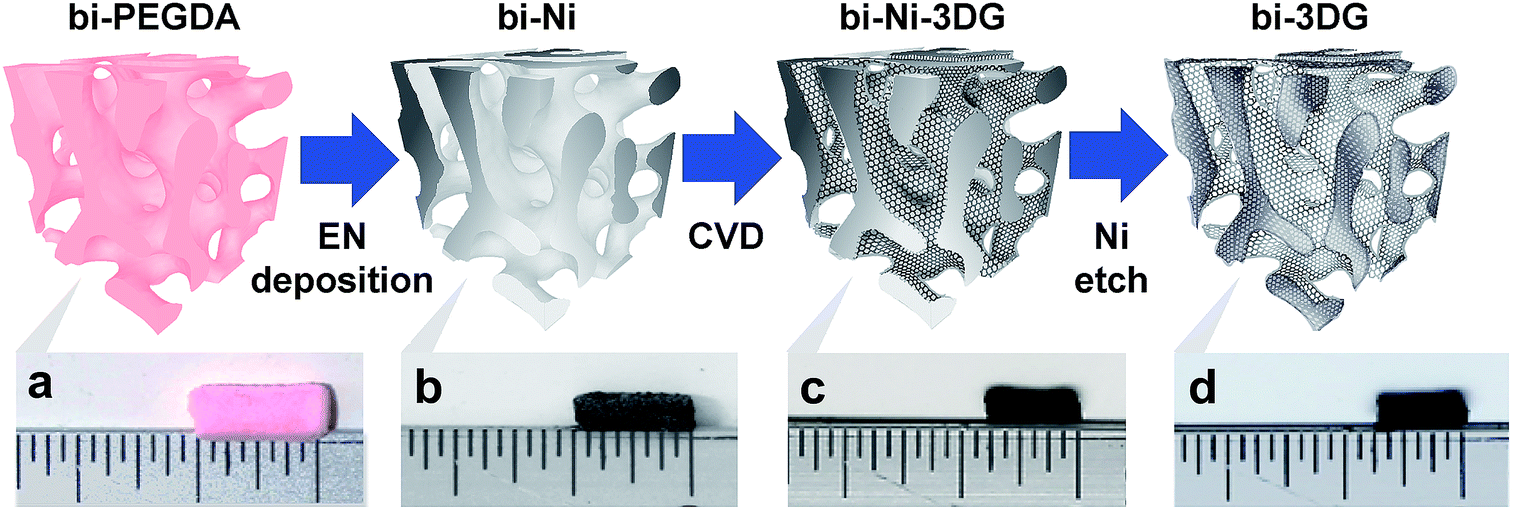
\includegraphics[scale = 0.5]{figures/introduction/bijel_templating.png}
    \caption{Fabrication of a graphite oxide battery electrode using bijel template. \cite{garcia_scalable_2019}}
    \label{fig:bijel_template}
\end{figure}

Conventionally, porous materials have been synthesized through solvothermal synthesis or pyrolysis used in the synthesis of zeolites and activated carbon respectively. With more targeted applications of porous materials, synthesis techniques such as sol-gel synthesis, freeze drying and various forms of templating have been utilized to synthesize porous materials from length scales of $10^{-9}m$ to $10^{-3}m$. \cite{stein_morphological_2008, ray_comprehensive_2016, cervellere_mesoscopic_2019, garcia-bennett_unique_2020, zhang_emulsion_2019, alves-rosa_design_2013} Industry has also taken up techniques such as electrospinning to generate non woven fibers, used in membrane synthesis. Templating techniques in particular offer access to various pore length scales, bottom up synthesis and functionality through leveraging various physical phenomena. Colloidal templating works through the close packing of particles. Surfactant and polymer templating work through the assembly of macromolecules into their equilibrium configurations. Emulsion templating utilizes the phase separation of partially misicble liquids to form the pore structure of a porous material. 

Emulsion templating offers access to a large length scale of tunable pore sizes, continous production through microfluidic junctions or other flow media, functionalization through the addition of additives or stabilizers, scope of accessible microstructures and mild synthesis conditions. It can further be extended to include heirarchical porosity, further enhancing its utility and fabricated material properties. \cite{yang_hierarchically_2017, thompson_hierarchically_2019, wang_morphology_2023} Figure \ref{fig:bijel_template} demonstrates how emulsion templating allows bottom up synthesis of hierarchically porous materials, although other examples do exist. \cite{garcia_scalable_2019, santiago_cordoba_aerobijels_2020, thorson_bijel-templated_2019, lu_controllable_2020, wang_morphology_2023}

\begin{figure}
    \centering
    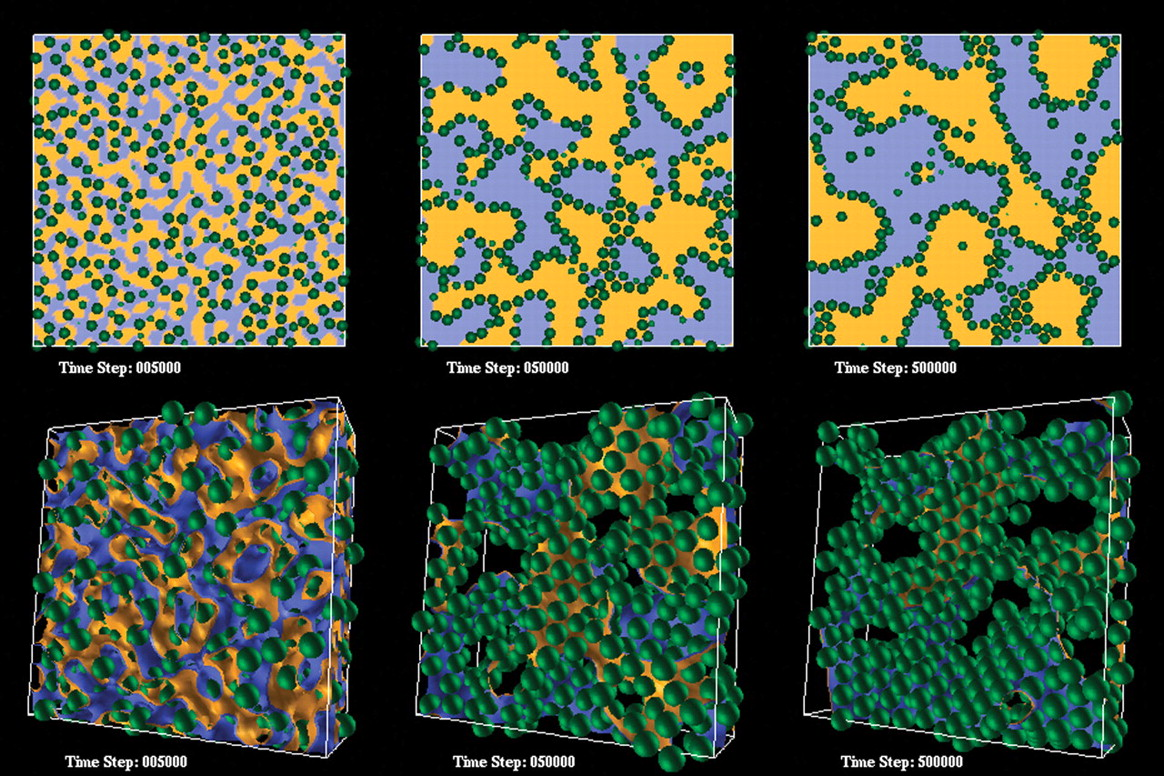
\includegraphics[scale = 0.3]{figures/introduction/bijel_coarsening.jpg}
    \caption{Initiation and arrest of spinodal decomposition as particles adsorb onto the interface, followed by jamming once the interfacial area matches the cross sectional area of the adsorbed particles\cite{stratford_colloidal_2005}}
    \label{fig:bijel_coarsen}
\end{figure}

One such emulsion microstructure of interest is the bicontinuous interfacially jammed emulsion gel(bijel). \cite{stratford_colloidal_2005, herzig_bicontinuous_2007, lee_bicontinuous_2010} Bijels are made by arresting the spinodal decomposition of partially miscible liquids, caused by particles adsorbing on the interface and jamming as the cross sectional area of the particles match that of the interface, summarized in Figure \ref{fig:bijel_coarsen}. Bijels are of interest due to their co-continuous, tortuous microstructure which represent excellent fits for several porous material applications.

Bijels were discovered in simulations in 2005 and experimentally realized in 2007 when a mixture of water and 2-6-lutidine mixed with surface modified silica nanoparticles underwent thermally induced spinodal decomposition. \cite{stratford_colloidal_2005, herzig_bicontinuous_2007} Since then, multiple other casting mixtures and particle chemistry's have been used to fabricate bijels using Thermally Induced Spinodal Decomposition (TIPS). \cite{lee_bicontinuous_2010, bai_dynamics_2015} More recently, techniques such as Solvent Transfer Induced Phase Separation (STrIPS), Vapor Induced Phase Separation (VIPS), Non-solvent Induced Phase Separation (NIPS), homogenization and liquid in liquid printing have been utilized to fabricate bijels, demonstrating the ability for bijels to be synthesized in a continuous process, suitable for scale up. \cite{haase_continuous_2015, wang_scalable_2020, cai_bijels_2017, yabuno_preparation_2020, wang_bicontinuous_2023, amirfattahi_fabrication_2024} These techniques also offer preparation of bijels in various different shapes and form-factors for various uses such as fibers, coatings and capsules, seen in Figure \ref{fig:strips}. \cite{haase_continuous_2015, boakye-ansah_controlling_2020, kharal_hightensile_2020, wang_bicontinuous_2023}

\begin{figure}[h]
    \centering
    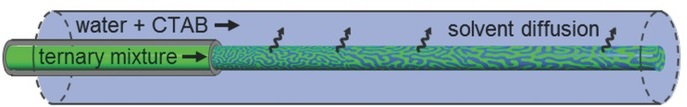
\includegraphics[scale = 2]{figures/literature_review/STRIPPS.jpg}
    \caption{STrIPS in action. Extrusion of the bijel casting mixture into a non-solvent bath, followed by removal of solvent from the casting mixture through diffusion. \cite{haase_continuous_2015}}
    \label{fig:strips}
\end{figure}

However, these techniques all depend upon controlling the rate of phase separation, which involve changing the casting mixture composition to modify the obtained microstructure. In STrIPS, the obtained bijel microstructure is a function of the flow rate and selected co-solvent, selected to change the rate of phase separation. \cite{haase_continuous_2015} This affects material properties such as the mechanical performance of the bijel, important in fields such as catalysis where rigidity of the particle monolayer is crucial in ensuring consistent performance. \cite{reeves_particle-size_2015, haase_situ_2016, boakye-ansah_controlling_2020} Identification of other techniques that can be utilized to modify the microstructure of a bijel would enable bijels to continue using the desired composition of constituents, while also adding other unique properties. Stimuli response offers one such road to microstructure modification.

\textcolor{blue}{ADD IN PICTURE FROM THAM 2021 AND CUI 2013 ON EXAMPLES OF STIMULI RESPONSE IN EMULSIONS}

Stimuli response based on pH, external fields and temperature have been used in past works when looking at modifying the microstructure of emulsion droplets for enhanced oil recovery, pharmaceutical and cell adhesion. \cite{haase_nanoparticle_2011, tham_magnetophoresis_2021, cui_stabilizing_2013, manfredini_limonene--water_2021}  It was shown that external fields can be used to move, control emulsion stability and elongate emulsion droplets. \cite{tham_magnetophoresis_2021, cui_stabilizing_2013} \textcolor{blue}{https://pubs.acs.org/doi/10.1021/la047691n} Bijels stabilized spherical particles under a magnetic field showed no meaningful microstructure changes. \cite{kim_bijels_2010} Bijels stabilized with spherical particles under an electric field showed more promise. \cite{carmack_tuning_2018} However, magnetic fields offer more targeted stimuli response, allowing even weak fields to incite a response. Magnetic fields non-interaction in many situations offer advantages to many of the desired uses of bijels within pharmaceutical or bioengineering applications. \cite{vanoli_bijels_2022, thorson_bijel-templated_2019, thorson_composite_2018} These same applications also have a need for in-situ microstructure modification that would enable tunable drug delivery rates, separations or catalyst efficiency and permeability improvements in the system. Therefore, identifying schemes that allow modification of the pore size and tortuosity  without synthesis of a new material would enhance the use case of bijels. 

Anisotropic particles at interfaces have shown self assembly due to the presence of multi-polar pressure fields caused by interface deformation. Self assembly has also been shown for ellipsoidal particles at interfaces under magnetic fields. Ellipsoidal particles have also been shown to exhibit magnetic field controlled orientations at interfaces, as Bresme and Faraudo showed. \cite{bresme_orientational_2007, davies_interface_2014} Under magnetic fields, assemblies of multiple ellipsoidal particles have been shown to have energy minima at unexpected locations. \cite{newton_influence_2014, newton_capillary_2018} Thus ellipsoidal particles at interfaces, whose orientations and packing can be controlled through external fields, offer a potential means to control the microstructure of bijels.

Bijels present a bottom up synthesis strategy for porous material templates for hard and soft material applications in a scalable and continuous method using STrIPS and other techniques. However, the microstructure control these techniques offer are intrinsically linked to the casting mixture composition. Stimuli response offers a way to modify the microstructure of bijels while still maintaining the various form factors these continuous synthesis techniques can output. While stimuli response has been explored in the past using bijels stabilized with spherical particles with little success, anisotropic particles are poised to allow microstructure modification of bijels upon application of an external field. This technique also has the potential to allow for post synthesis microstructure modification. Therefore, this work seeks to identify a means to control the microstructure of a bijel stabilized with magnetically responsive ellipsoidal particles using magnetic fields.

% Bijels have proposed uses in many of these with the microstructure of the material being shown to affect material properties. \cite{cha_bicontinuous_2019, khan_nanostructured_2022, vanoli_bijels_2022} 

% Magnetic fields offer several advantages over currently utilized techniques such as electric fields and shear. \cite{cui_stabilizing_2013, mulligan_deformation_2011} These include greater specificity of response as most materials are unresponsive to magnetic stimuli as well as even weak fields being sufficient to incite responses in many cases.

% this adds value to many of the desired uses of bijels within pharmaceutical or bioengineering applications. \cite{vanoli_bijels_2022, thorson_bijel-templated_2019, thorson_composite_2018}

\textcolor{blue}{Add commentary about past results with bijels and why we use anisotropic particles in bijels. Changes this makes} Therefore, identification of a scheme which allows for tunability of the microstructure, independent of the composition of the casting mixture and post synthesis is the goal of this work.

\section{Research objective}

This work seeks to identify means to control the bijel microstructure independent of the casting mixture composition by utilizing magnetic stimuli on bijels stabilized with magnetically responsive ellipsoidal particles. The proposed mechanism of microstructure modification is driven through reorientation of the particles to the applied magnetic field altering how the particles pack on the interface. By changing the interfacial packing of the particles, we change when the particles jam, which in turn changes the jamming point of the bijel. This mechanism is predicted to be effective during and after synthesis. The processability of bijels fabricated using this technique will also be investigated to ascertain how changes in particle packing affect the rheology of the material. An overview of three major research aims will be presented below.

% this work seeks to identify means to control the bijel microstructure independent of the casting mixture composition utilizing magnetic stimuli response of anisotropic particles. The proposed mechanism of microstructure modification is driven through reorientation of the particles to the applied magnetic field altering how the particles pack on the interface.

\subsection{Aim 1: Determination of the degree of microstructure changes expected when applying a constant field during bijel formation}
\label{section:aim1_desc}

The jamming point of a bijel controls the obtained microstructure, as shown by previous work comparing the length scale of bijels synthesized with different particle volume fractions. It has also been shown how magnetic fields can be used to self assemble ansisotropic particles at interfaces and how they can tilt out of the interface. \cite{davies_interface_2014, davies_assembling_2014} On a curved interface with many other particles, it is unknown how multiple particles orienting to a field and having regular structure will affect when and how the bijel will jam. \cite{bresme_orientational_2007, davies_interface_2014}

To assess the obtained microstructure upon application of a field during formation of the bijel, homogenous mixtures containing spherical and ellipsoidal particles will be subjected to field strengths above and below the critical field strength when particle orientations to the interface are controlled by the applied field strength, as calculated by Bresme and Faraudo for the particle used. This selection of fields will allow insight into the controlling mechanisms behind microstructural changes observed, allowing verification of the hypothesis and ascertainment where the most control over the microstructure can be exercised.

The average and directional domain sizes in addition to their relation with tortuosity will provide windows into the microstructural properties of the resulting bijel. The nematic order parameter and average interfacial angle will be used to investigate how the application of the field affects the particle ordering to each other, and to the interface. Finally, the radial distribution function will be used to assess if the orientational changes expected upon field application, affects the packing of the particles on the interface.

\subsection{Aim 2: Microstructure changes and timescales upon application of a magnetic field after formation}
\label{section:aim2_desc}

Particles on the surface of emulsion droplets have been shown to unjam and rejam into new, stable microstructures upon application of stimuli. \cite{cui_stabilizing_2013} Two techniques of microstructure change are proposed. The first technique is that the adsorption energy is so strong that the interface is dragged along with the particles until they rejam in their new location and orientation to the field. The second technique is that the particles tilt in place out of the interface, causing domain coarsening before the particles jam in their new positions and orientations. The mechanism, derived microstructure change and timescales will be assessed in this aim.

The response of bijels to magnetic fields will be assessed through analyzing how model bijels made with no fields respond to field strengths above and below the critical field strength as calculated from Bresme Faraudo theory. The microstructure properties such as the average domain size, particle orientation to the field and interface and the Steinhardt 6 fold bond order parameter to examine the spatial relationship of the particles to their neighbors. These techniques will allow elucidation of which mechanism is present at which magnetic field strength. Additionally, the microstructure changes observed will be characterized and compared to one another to assess how the applied magnetic field changes the final microstructure obtained. 

Next, the importance of the initial order of the particle monolayer will also be assessed through increasing the applied field to equal to the surface tension forces on bijel templates simulated under various field strengths. The applied field will also be switched off on bijel templates simulated under the same field strengths. The same analysis metrics mentioned earlier will be used. Additionally, the microstructures with the same difference in applied field,  will be assessed to investigate the reversibility of bijel microstructures. 

\subsection{Aim 3: Rheological characterization of bijels formed under and subjected to a magnetic field}
\label{section:aim3_desc}

In many of the fabrication processes described above, the rheology of the bijel casting mixture is essential. \cite{haase_continuous_2015, cai_bijels_2017, amirfattahi_fabrication_2024} Ching showed that rheologically, bijels are colloidal glasses percolating in 3D space. \cite{ching_bijel_2022} First, a shear capillary number is defined as $Ca_s = \frac{\eta_{f} \dot{\gamma} L_{1}}{\sigma}$ where $\dot{\gamma} = \frac{u_{LE}}{L_x}$ is the strain rate and $L_1$ is the average domain size. \cite{frijters_effects_2012, yang_capillary_2022} Lower capillary numbers in the range of $ 10^{-7} \geq Ca_s \leq 10^{-5}$ will be utilized. 
% which corresponds to a $Ma << 0.01$ to accommodate the hydrodynamic model utilized.

For this study, the yield stress and viscosity of the bijels will be explored as a function of the initial microstructure under various $Ca_s$. Four templates with different processing history will be utilized to assess the impact of initial microstructure on the obtained rheology. These are, $\bar{B} = 0$, $\bar{B} = 1$, $\bar{B} = 0 \rightarrow \bar{B} = 1$ and $\bar{B} = 1 \rightarrow \bar{B} = 0$. To explain any observed differences in the the yield stress and viscosity, the time evolution of the domain size, average interface angle, and nematic order parameter will be characterized and compared to the observed yield stress and viscosity. Additionally, the presence of shear banding will be visually confirmed.